\begin{center}
	\Large\textbf{{{Реализация граничных и контактных условий при использовании 
	сеточно-характеристического метода (СХМ) на неструктурированных расчётных сетках}}}
\end{center}

\section{Система уравнений}
В произвольной $D$-мерной области ($D = 2, 3$) решается система уравнений 
в частных производных гиперболического типа:
\begin{equation}
\label{general_equation}
	\frac{\partial\vec{u}}{\partial{t}}+
	\mathbf{A}_1\frac{\partial\vec{u}}{\partial{x_1}}+...+
	\mathbf{A}_D\frac{\partial\vec{u}}{\partial{x_D}}=0.
\end{equation}
Здесь $\{x_1, ..., x_D\}$ -- ортонормированный базис, 
$\vec{u}$ -- вектор неизвестных размерности $N$,
матрицы $\mathbf{A}_i$ считаются постоянными.
Кроме того, ставятся начальные условия -- значения $\vec{u}$ 
во всей области решения в нулевой момент времени и
граничные условия -- некоторое количество условий на $\vec{u}$ 
на границе области решения в любой момент времени.

Конкретный вид матриц и физический смысл уравнений можно не уточнять. 
Единственное условие -- матрицы должны быть диагонализуемы с полным набором 
собственных векторов, и для каждого ненулевого собственного значения должно быть
равное по модулю с противоположным знаком. Эти требования означают, фактически,
то, что система уравнений описывает некоторый волновой процесс. Количество
независимых скалярных граничных условий на $\vec{u}$ равно количеству
положительных (отрицательных) собственных значений матрицы $\mathbf{A}_i$, 
которое в дальнейшем обозначим за $M$.


\section{Численный метод}
В наиболее общей постановке и с иллюстрацией множества приложений 
СХМ изложен его создателями в \cite{magomedov_kholodov_1988}. 
К двумерным волновым уравнениям механики упругого тела 
СХМ впервые применён в \cite{petrov_kholodov}.
Основная идея реализации метода на неструктурированных расчётных сетках, 
в том числе граничных и контактных условий предложена в 
\cite{magomedov_kholodov_1988} и в \cite{chelnokov}.

\subsection{Неструктурированная расчётная сетка}
Для возможности применения метода к областям произвольной формы используются
треугольные и тетраэдральные неструктурированные расчётные сетки, для построения
которых использовались в основном библиотеки CGAL \cite{cgal} и Ani3D \cite{ani3d}.
Значения искомой функции хранятся в узлах сетки. 

Подразумевается, что внутри каждой области интегрирования матрицы $\mathbf{A}_i$
постоянны. Для моделирования неоднородностей явно выделяются дополнительные
области, между которыми рассчитывается контакт.

Стоит отметить, что метод реализации граничных и контактных условий не закладывается на 
топологию ячейки сетки, то есть может быть применён, к примеру, и к октаэдрическим сеткам.

\subsection{Расщепление по направлениям}
Поскольку СХМ в чистом виде рассматривает только одномерные уравнения,
для численного решения \eqref{general_equation} необходимо
перейти к решению одномерных систем уравнений -- так называемое расщепление по направлениям:
\begin{equation}
\label{equation_1d}
	\frac{\partial\vec{u}}{\partial{t}}+\mathbf{A_i}\frac{\partial\vec{u}}{\partial{\xi_i}} = 0, \quad i = 1 ... D.
\end{equation}
Здесь под $\{\xi_i\}$ подразумевается произвольный ортонормированный базис, 
не обязательно совпадающий с $\{x_i\}$ (вид матриц $\mathbf{A_i}$, конечно, зависит от базиса).

В данной работе используется предложенная в \cite{chelnokov}
экономичная по памяти и вычислительным ресурсам схема расщепления, 
обладающая при этом близким ко второму порядком точности по времени.
Полный шаг по времени $\tau$ решения многомерного уравнения \eqref{general_equation} состоит из $D$ 
последовательных ступеней, $i$-я ступень заключается в выполнении шага по времени
для $i$-го уравнения \eqref{equation_1d} на то же время $\tau$. В качестве значений
старого временного слоя для каждой последующей ступени берётся результат выполнения
предыдущей, а результат выполнения последней ступени является решением 
многомерного уравнения на новом временном слое. 


\subsection{Решение одномерного уравнения}
По условию матрицы $\mathbf{A}_i$ диагонализуемы с полным набором собственных векторов:
\begin{equation}
	\label{diagonal_view}
	\mathbf{A} = \mathbf{U}^{-1}\mathbf{\Lambda}\mathbf{U}.
\end{equation}
Здесь $\mathbf{U}^{-1}$ -- матрица собственных векторов, 
$\mathbf{\Lambda}$ -- диагональная матрица собственных значений,
$\mathbf{U}$ -- матрица собственных строк.
Умножив \eqref{equation_1d} слева на $\mathbf{U}$, 
внеся постоянную матрицу $\mathbf{U}$ под знак дифференциала
и обозначая $\vec{r} = \mathbf{U}\vec{u}$ -- инварианты Римана, получаем:
\begin{equation}
	\label{in_riemann_invariants}
	\frac{\partial\vec{r}}{\partial{t}}+\mathbf{\Lambda}\frac{\partial\vec{r}}{\partial{x}} = 0.
\end{equation}
В новых переменных система распалась на независимые уравнения переноса.
Их численное решение заключается в интерполяции значения функции
на предыдущем временном слое в точке, где характеристика из узла 
на новом временном слое пересекает предыдущий. 
После переноса инвариантов с предыдущего временного слоя на новый
производится обратная замена переменных $\vec{u} = \mathbf{U}^{-1}\vec{r}$.
Сказанное проиллюстрированно на рисунке \ref{pic:gcm-idea}.
\begin{figure}[H]
	\center{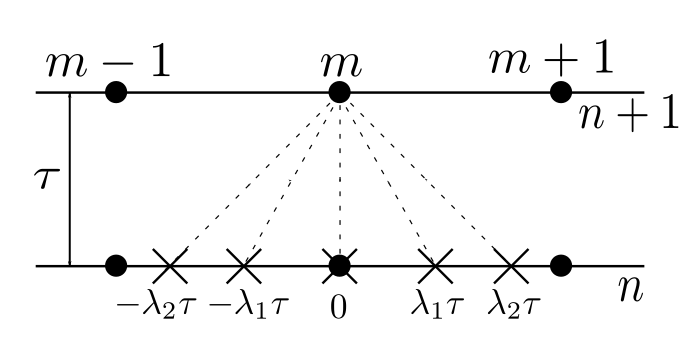
\includegraphics[width=0.5\textwidth]{gcm-idea.png}}
	\caption{Основная идея сеточно-характеристического метода}
	\label{pic:gcm-idea}
\end{figure}

\begin{figure}[H]
	\center{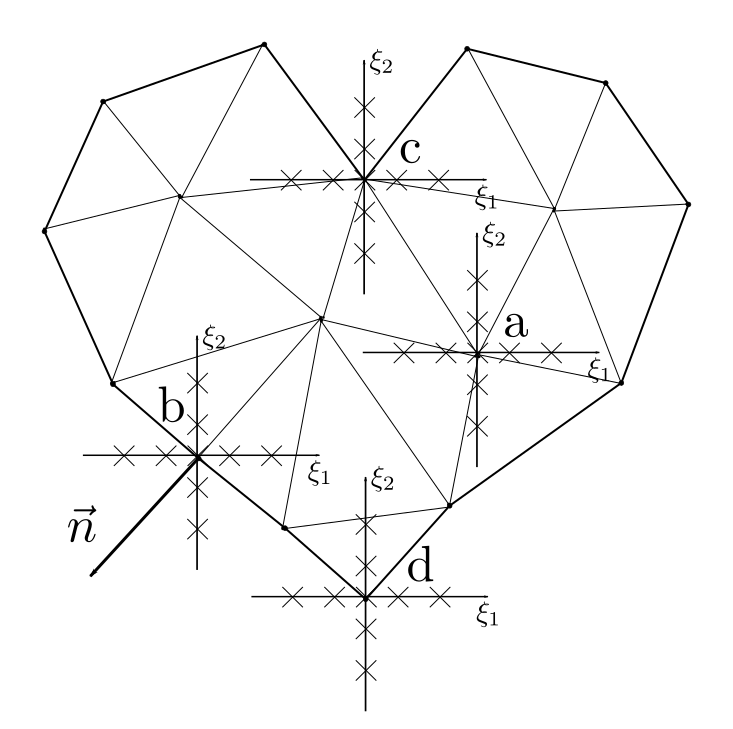
\includegraphics[width=0.5\textwidth]{gcm-on-triangles.png}}
	\caption{Иллюстрация сеточно-характеристического метода на треугольной расчётной сетке}
	\label{pic:gcm-idea}
\end{figure}


\subsection{Общая схема метода на границе области интегрирования}
Описанный выше алгоритм пригоден для внутренних узлов, когда все выброшенные 
из узла характеристики пересекают предыдущий временной слой внутри области интегрирования.
Для граничных и контактных узлов, когда часть характеристик ``выпадает'' за границу 
(назовём их внешними характеристиками), 
применяется его модификация, называемая коррекцией внешними волнами 
(то есть волнами, соответствующими инвариантам Римана, характеристики которых оказались внешними).

Запись произвольного линейного граничного условия для произвольной модели:
\begin{eqnarray}
\label{boundary_condition}
	\mathbf{B} \cdot \vec{u} = \vec{b}.
\end{eqnarray}
Здесь $\mathbf{B}$ -- матрица размерности $M \times N$, $\vec{b}$ -- вектор размерности $M$, 
определяющие собой конкретный вид граничного условия.

На первом этапе делается расчёт граничных узлов по алгоритму для внутренних, 
при этом все инварианты Римана, соответствующие внешним характеристикам, приравниваются к нулю. 
Получается $\vec{u}^{inner}$. Затем выполняется граничная коррекция -- 
добавление такой линейной комбинации внешних волн, 
которая обеспечит выполнение граничного условия \eqref{boundary_condition}:
\begin{eqnarray}
	\mathbf{B} \cdot (\vec{u}^{inner} + \mathbf{\Omega} \cdot \vec{\alpha}) = \vec{b}.
\end{eqnarray}
Здесь $\mathbf{\Omega}$ -- матрица, в столбцах которой стоят собственные векторы 
матрицы $\mathbf{A}$, соответствующие внешним характеристикам, 
$\vec{\alpha}$ -- коэффициенты в линейной комбинации, которые нужно определить.

Для определения коэффициентов $\vec{\alpha}$ необходимо решить 
СЛАУ с матрицей $\mathbf{B} \mathbf{\Omega}$ размерностью $M \times M$:
\begin{eqnarray}
	\mathbf{B} \mathbf{\Omega} \cdot \vec{\alpha} = \vec{b} - \mathbf{B} \cdot \vec{u}^{inner}.
\end{eqnarray}

После определения коэффициентов линейной комбинации производится собственно коррекция:
\begin{eqnarray}
\vec{u}^{n+1} = \vec{u}^{inner} + \mathbf{\Omega} \cdot \vec{\alpha}
\end{eqnarray}


\subsection{Общая схема метода на контакте двух областей интегрирования}
Запись произвольного линейного контактного условия для произвольных моделей:
\begin{eqnarray}
\label{contact_condition}
\begin{split}
	\mathbf{B}_{1A} \cdot \vec{u}_A = \mathbf{B}_{1B} \cdot \vec{u}_B, \\
	\mathbf{B}_{2A} \cdot \vec{u}_A = \mathbf{B}_{2B} \cdot \vec{u}_B.
\end{split}
\end{eqnarray}
Здесь обозначения те же, что и в \eqref{boundary_condition}.

Все действия аналогичны расчёту граничных узлов. 
Сначала делается расчёт контактных узлов в обоих телах по алгоритму для внутренних.
Получается ${\vec{u}_A}^{inner}$ и ${\vec{u}_B}^{inner}$. 
Затем выполняется контактная коррекция -- 
добавление в обоих узлах такой линейной комбинации внешних волн, 
которая обеспечит выполнение контактного условия \eqref{contact_condition}. 

Распишем сообразно сказанному условие \eqref{contact_condition}:
\begin{eqnarray}
	\mathbf{B}_{1A} \cdot ({\vec{u}_A}^{inner} + \mathbf{\Omega}_A \cdot \vec{\alpha}_A) = \mathbf{B}_{1B} \cdot ({\vec{u}_B}^{inner} + \mathbf{\Omega}_B \cdot \vec{\alpha}_B), \\
\label{second_line_in_contact_condition_wide}
	\mathbf{B}_{2A} \cdot ({\vec{u}_A}^{inner} + \mathbf{\Omega}_A \cdot \vec{\alpha}_A) = \mathbf{B}_{2B} \cdot ({\vec{u}_B}^{inner} + \mathbf{\Omega}_B \cdot \vec{\alpha}_B).
\end{eqnarray}

Раскроем скобки:
\begin{eqnarray}
	(\mathbf{B}_{1A} \mathbf{\Omega}_A) \cdot  \vec{\alpha}_A = \mathbf{B}_{1B} \cdot {\vec{u}_B}^{inner} - \mathbf{B}_{1A} \cdot {\vec{u}_A}^{inner} + (\mathbf{B}_{1B} \mathbf{\Omega}_B) \cdot \vec{\alpha}_B
\end{eqnarray}

Сделаем переобозначения:
\begin{align}
\label{matrixRcontact}
\mathbf{R} &= (\mathbf{B}_{1A} \mathbf{\Omega}_A)^{-1}, &\\
\vec{p} &= \mathbf{R} \cdot (\mathbf{B}_{1B} \cdot {\vec{u}_B}^{inner} - \mathbf{B}_{1A} \cdot {\vec{u}_A}^{inner}), &\\
\mathbf{Q} &= \mathbf{R} \cdot (\mathbf{B}_{1B} \mathbf{\Omega}_B).
\end{align}

Тогда:
\begin{eqnarray}
\label{alpha_A_from_B}
\vec{\alpha}_A = \vec{p} + \mathbf{Q} \cdot \vec{\alpha}_B.
\end{eqnarray}

Подставляем в \eqref{second_line_in_contact_condition_wide}:
\begin{eqnarray}
\begin{split}
\mathbf{B}_{2A} \cdot {\vec{u}_A}^{inner} + (\mathbf{B}_{2A} \mathbf{\Omega}_A) \cdot \vec{p} + (\mathbf{B}_{2A} \mathbf{\Omega}_A) \cdot \mathbf{Q} \cdot \vec{\alpha}_B = \\ =
\mathbf{B}_{2B} \cdot {\vec{u}_B}^{inner} + (\mathbf{B}_{2B} \mathbf{\Omega}_B) \cdot \vec{\alpha}_B.
\end{split}
\end{eqnarray}

Получаем СЛАУ на $\vec{\alpha}_B$:
\begin{eqnarray}
\label{SLE_on_alphaB}
\begin{split}
\Bigg[  (\mathbf{B}_{2B} \mathbf{\Omega}_B) - (\mathbf{B}_{2A} \mathbf{\Omega}_A) \cdot \mathbf{Q}  \Bigg] \cdot \vec{\alpha}_B = \\ = 
(\mathbf{B}_{2A} \mathbf{\Omega}_A) \cdot \vec{p} + \mathbf{B}_{2A} \cdot {\vec{u}_A}^{inner} - \mathbf{B}_{2B} \cdot {\vec{u}_B}^{inner}.
\end{split}
\end{eqnarray}

Решив систему на $\vec{\alpha}_B$, находим $\vec{\alpha}_A$ из \eqref{alpha_A_from_B}.

После чего производим собственно коррекцию:
\begin{eqnarray}
{\vec{u}_A}^{n+1} = {\vec{u}_A}^{inner} + \mathbf{\Omega}_A \cdot \vec{\alpha}_A, \\
{\vec{u}_B}^{n+1} = {\vec{u}_B}^{inner} + \mathbf{\Omega}_B \cdot \vec{\alpha}_B
\end{eqnarray}

Для проведения изложенных вычислений необходимо 
сначала один раз обратить матрицу размерностью $M \times M$ в \eqref{matrixRcontact}, 
а затем решить СЛАУ \eqref{SLE_on_alphaB} с матрицей той же размерности.


\subsection{Вырождение матрицы СЛАУ граничного и контактного корректора}

\subsubsection{необходимость согласованности ну и гу}



====== Плохие граничные, контактные и мультиконтактные случаи, принципиальное ограничение метода
====== Усложнение при некурантовском шаге (и его необходимость в 3D)
====== Интерполяция без доп.узлов (надо ли?)
====== Поиск точки (надо ли?)

\section{Результаты}


\begin{thebibliography}{9}
\addcontentsline{toc}{section}{Литература}

\bibitem{magomedov_kholodov_1988} Магомедов К.М., Холодов А.С. 
Сеточно-характеристические численные методы. — М.: Наука, 1988, 288 с.

\bibitem{petrov_kholodov} Петров И.Б., Холодов А.С. 
Численное исследование некоторых динамических задач механики деформируемого 
твёрдого тела сеточно-характеристическим методом, 
Ж. вычисл. матем. и матем. физ., 24:5 (1984), 722–739.

\bibitem{chelnokov} Челноков Ф.Б., Явное представление 
сеточно-характеристических схем для уравнений упругости в двумерном и
 трехмерном пространствах, Матем. моделирование, 18:6 (2006), 96–108.

\bibitem{cgal} CGAL, Computational Geometry Algorithms Library, http://www.cgal.org

\bibitem{ani3d} 3D generator of anisotropic meshes http://sourceforge.net/projects/ani3d

\end{thebibliography}














